% !Rnw weave = knitr
\documentclass[11pt]{article}\usepackage[]{graphicx}\usepackage[]{color}
% maxwidth is the original width if it is less than linewidth
% otherwise use linewidth (to make sure the graphics do not exceed the margin)
\makeatletter
\def\maxwidth{ %
  \ifdim\Gin@nat@width>\linewidth
    \linewidth
  \else
    \Gin@nat@width
  \fi
}
\makeatother

\definecolor{fgcolor}{rgb}{0.345, 0.345, 0.345}
\newcommand{\hlnum}[1]{\textcolor[rgb]{0.686,0.059,0.569}{#1}}%
\newcommand{\hlstr}[1]{\textcolor[rgb]{0.192,0.494,0.8}{#1}}%
\newcommand{\hlcom}[1]{\textcolor[rgb]{0.678,0.584,0.686}{\textit{#1}}}%
\newcommand{\hlopt}[1]{\textcolor[rgb]{0,0,0}{#1}}%
\newcommand{\hlstd}[1]{\textcolor[rgb]{0.345,0.345,0.345}{#1}}%
\newcommand{\hlkwa}[1]{\textcolor[rgb]{0.161,0.373,0.58}{\textbf{#1}}}%
\newcommand{\hlkwb}[1]{\textcolor[rgb]{0.69,0.353,0.396}{#1}}%
\newcommand{\hlkwc}[1]{\textcolor[rgb]{0.333,0.667,0.333}{#1}}%
\newcommand{\hlkwd}[1]{\textcolor[rgb]{0.737,0.353,0.396}{\textbf{#1}}}%
\let\hlipl\hlkwb

\usepackage{framed}
\makeatletter
\newenvironment{kframe}{%
 \def\at@end@of@kframe{}%
 \ifinner\ifhmode%
  \def\at@end@of@kframe{\end{minipage}}%
  \begin{minipage}{\columnwidth}%
 \fi\fi%
 \def\FrameCommand##1{\hskip\@totalleftmargin \hskip-\fboxsep
 \colorbox{shadecolor}{##1}\hskip-\fboxsep
     % There is no \\@totalrightmargin, so:
     \hskip-\linewidth \hskip-\@totalleftmargin \hskip\columnwidth}%
 \MakeFramed {\advance\hsize-\width
   \@totalleftmargin\z@ \linewidth\hsize
   \@setminipage}}%
 {\par\unskip\endMakeFramed%
 \at@end@of@kframe}
\makeatother

\definecolor{shadecolor}{rgb}{.97, .97, .97}
\definecolor{messagecolor}{rgb}{0, 0, 0}
\definecolor{warningcolor}{rgb}{1, 0, 1}
\definecolor{errorcolor}{rgb}{1, 0, 0}
\newenvironment{knitrout}{}{} % an empty environment to be redefined in TeX

\usepackage{alltt}
\usepackage[backend=biber, sorting=nyt, maxcitenames=2, doi=false,url=false, style=apa]{biblatex} %add annotation=true and style=reading to print the annotations in the bibliography
\usepackage[american]{babel}
%\usepackage{newtxtext,newtxmath}
\usepackage{csquotes}
\bibliography{/home/harold/Dropbox/full,/home/harold/github/eysterthesis/manuscript/thesis_ref}
\DeclareLanguageMapping{american}{american-apa}
\usepackage[compact]{titlesec}
\usepackage{csquotes}
\usepackage{amsmath}
%\usepackage[hyphens]{url}
\usepackage[margin=1in]{geometry}
\usepackage{mathtools}
\setlength{\parskip}{.6em}
\usepackage{setspace}
\doublespacing
\usepackage{multicol}
\usepackage{longtable}
\usepackage{makecell}
\renewcommand\theadalign{bc}
\renewcommand\theadfont{\bfseries}
\renewcommand\theadgape{\Gape[4pt]}
\renewcommand\cellgape{\Gape[4pt]}
\renewcommand{\tablename}{Table}
%\usepackage{sectsty}
%\allsectionsfont{\singlespacing}
%\usepackage{indentfirst} %This indents the pfaragraph following a heading 
\setlength{\parindent}{0em}
\usepackage{breqn}
\usepackage{xr} % run xelatex, then pdflatex.
\externaldocument{SI}
\usepackage{graphicx}
\usepackage{pdfpages}
\usepackage{subcaption}
\usepackage[figuresleft]{rotating}
\usepackage{lineno}
\graphicspath{{home/harold/github/eysterthesis/manuscript/}} %make sure to include the slash after the colon at at the end 
%Make sure Bibliography --> is set as biblatex 
%Then run tools-->bibliography, then compile 
\usepackage{authblk}
%\title{Comparisons in the native and introduced ranges reveal little evidence of climatic adaptation in germination traits}
%\author[1,2,3,*]{Harold N. Eyster}
%\author[2,3,4]{Elizabeth M. Wolkovich}
%\affil[1]{Institute for Resources, Environment, and Sustainability, University of British Columbia, 429-2202 Main Mall, Vancouver, BC, Canada V6T 1Z4}
%\affil[2]{Arnold Arboretum of Harvard University, 1300 Centre Street, Boston, MA 02130, USA}
%\affil[3]{Department of Organismic \& Evolutionary Biology, Harvard University, 26 Oxford Street, Cambridge, MA 02138,USA}
%\affil[4]{Department of Forest and Conservation Science, University of British Columbia, 3041-2424 Main Mall, Vancouver, BC, Canada V6T 1Z4 }
%\affil[*]{Corresponding author. haroldeyster@gmail.com}
%\date{}                     %% if you don't need date to appear
%\setcounter{Maxaffil}{0}
%\renewcommand\Affilfont{\itshape\small}
\usepackage[export]{adjustbox}






\IfFileExists{upquote.sty}{\usepackage{upquote}}{}
\begin{document}
%\maketitle
%	\fbox{\includegraphics[width=1 \textwidth,trim=0cm 0cm 0cm 0cm, clip=true]{comps_overview}}
\linenumbers
%\begin{spacing}{1} %1.9
	\begin{abstract} 
Plant invasions are increasing due to globalization and environmental change, including through anthropogenic climate change. Yet we lack an understanding of how some species become widespread invaders while others do not. Two competing mechanisms have been posited: 1) post-introduction rapid evolution to the novel environments of the introduced range and 2) broad environmental tolerance in the source population that makes invaders tolerant of diverse introduced environments. Each mechanism has implications for how invaders respond to climate change: either needing to evolve to future climates, or already being tolerant of diverse current/future climates. Disentangling these mechanisms requires investigating how evolution versus tolerance drive essential invasion traits (germination rate and timing; growth rate). Here, we tested for evidence of rapid evolution in these traits by using growth chambers to provide common climates for seven herbaceous plant species sampled from multiple populations in their native (European) and invasive (North American) ranges. Chambers provided two levels of stratification—to simulate different winter lengths—and four temperature levels post-stratification—to simulate different spring conditions. We used Bayesian multilevel models to examine responses, while controlling for population and seed family. Across all species, trait responses were largely similar between native and invasive populations, except in response to particular climates representing cold winters and warm springs. Our results suggest that broad environmental tolerance, not rapid evolution, likely underlies invasion success for these invaders—and may sustain their spread with continued warming—but suggests that species may evolve to specific combinations of winter and spring climatic regimes.
	\end{abstract}
%\end{spacing}		
Keywords: Climate change ecology, Invasion ecology, Rapid evolution, Broad environmental tolerance, Phenology, Plant-climate interactions, Growth chamber experiment, Germination, Bayesian multilevel models, Invasive plants.
	\section{Introduction} 
	Exotic plant invasions  can transform biodiversity and ecosystems \parencite{Bellard2016, Pejchar2009,Mack2000}. %, and ecosystem function, services, and resilience \parencite{Bellard2016,Clavero2005,Walker1997,Daehler1999,Ehrenfeld2003,Wilcove1998,Pejchar2009,Pimentel2005,Pysek2010,OTA1993,Mack2000,Levine2003}.
These invasions are likely increasing: globalization is facilitating extra-range plant dispersal \parencite{Helmus2014}, and human alteration of ecosystems may provide new niche space \parencite{Tilman2001, Blois2013,Inouye2008,Harte2015}. Upon dispersing to a new environment, invasive species can thrive by filling vacant niches \parencite{Elton1958} or outperforming native plants in high-resource and variable environments \parencite{Davis2001,Daehler2003}. 

Changing environments, especially with anthropogenic climate change, could select for species that can take advantage of newly created temporal niches \parencite{Wolkovich2011,godoy2014}, and related resources, through shifts in the timing of flowering, fruiting, and other life history events \parencite{Franks2007}. Recent research shows invaders generally show differing sensitivity to climate \parencite{Reeb2020} and are  able to shift their phenology more than native species in their introduced communities \parencite{Wolkovich2014,Reeb2020,Zettlemoyer2019}. But how these invaders are more phenologically flexible has not been well studied. % Thus, disentangling the underlying drivers of plant invasion is becoming increasingly important with climate change. 

Two major biological mechanisms for how plants become widespread in novel environments are particularly relevant to understanding how phenology and invasions may intersect: 1) post-introduction rapid evolution and 2) broad environmental tolerance in the source population. A large body of literature supports this first mechanism of rapid evolution \parencite[e.g.,][]{Reznick2001, Prentis2008,Colautti2015,Lee2002invasion,Clements2011}.  Rapid evolution can enable nonindigenous species to adapt to vacant niches and take advantage of variable and high-resource environments, including by evolving greater competitive ability when released from natural enemies \parencite{Blossey1995,Bossdorf2005} or by evolving adaptive plasticity \parencite{Richards2006}. % %EMW8Apr -- suggest you cut this next sentence. you can bring it up in discussion if critical ... Many genetic characteristics have been identified to enable invasion, including additive genetic variation, epistasis, hybridization, genomic rearrangements, etc. \parencite[Reviewed in][]{Lee2002invasion}, while genetic drift and bottlenecks likely stifle invasion capacity \parencite{Bock2015}. 
%To invade new The first factor for determining invasion potential is dispersal. To become invasive, a species first needs a dispersal mechanism to establish in a non-native habitat \parencite{Mark2001,Westphal2008}. Humans have played an important role in facilitating recent plant dispersals \parencite{McKinney1999,Pysek2002,Vitousek1996}, and with increased globalization the spread of species outside their respective native ranges will only increase \parencite{Helmus2014}. Once a species is introduced to a novel region, however, it must also be able to successfully disperse beyond the initial introduction location to be considered fully invasive. Thus species with greater dispersal ability may be more successful invaders.  Nonetheless, any intrinsic biological dispersal advantage can be wholly dominated by intentional introduction, e.g., for agricultural or ornamental purposes, or by accidental human-facilitated mechanisms, such as the transportation of invasive species within contaminated mulch or gravel \parencite{Wittenberg2001}. 	
	%Managing this onrush of invasive species requires understanding the mechanisms that give some plants the capacity to exploit invasible environments \parencite{Hulme2013}
	
	
%	There are many examples of post-introduction rapid evolution abetting plant invasions. Genetic studies of two North American herbaceous goldenrods that invaded Europe, \textit{Solidago altissima} and \textit{S. gigantea} (Asteraceae), showed post-introduction genetic changes in flowering time in response to spring temperature, due to selection on source-population genetic variation and development of new mutations \parencite{Weber1998}. %Similarly, the invasive \textit{Centaurea solstitialis} (Asteraceae) in California evolved larger size from standing variation in the founding population \parencite{Barker2017}. 
    For example, a study found that genetic adaptation drove adaptive phenotypic variation in flowering time between high-altitude and desert populations of \textit{Capsella bursa-pastoris} (Brassicaceae) in California \parencite{Linde2001}. Invasion may even produce evolution sufficient to establish reproductive isolation and trigger speciation, in as few as 13 generations \parencite{Hendry2000}. If post-introduction rapid evolution is this central to invader success, it would have important implications for invasive species management: managers should treat invasives not as static, homogeneous species, but as constantly adapting populations \parencite{Lee2002invasion}. It would also suggest invaders will continually evolve with climate change and thus estimates of their responses today may not forecast their future climatic responses. 
	
	Yet, despite the support for the importance of post-introduction rapid evolution for widespread invaders, a competing body of literature suggests that invaders need not evolve to become widespread in novel environments. Instead, broad environmental tolerance, plasticity, weediness, and generalist adaptations to human-dominated environments within the source population may give invaders sufficient advantages to become widespread, obviating the necessity of post-introduction rapid evolution \parencite{Richards2006,Schwartz1994,Bock2015,Rejmanek1996,Baker1965}. A meta-analysis of 117 studies found that invasive plants were associated with general performance-related traits, and concluded that it may be possible to predict future invaders by those traits \parencite{VanKleunen2010}. %This is an longstanding theory. In 1965, Baker suggested that there were stable characteristics that made some species invasive: r-selected, high growth rates, broad environmental tolerance, etc. 
	%Studies have found contrasting results regarding whether weediness in the native range is the best predictor of widespread invasiveness %.  weedy in their native range are likely to be invasive in novel environments: a study of 274 plant species native to North and South America but naturalized in France showed that the best determinant of invasiveness was weediness in the home range
	%\parencite[e.g.,][]{Maillet2000}, or not \parencite{Perrins1992,Mack1996}. Seeking a unified answer, a meta-analysis of 117 studies found that invasive plants were associated with performance-related traits, and concluded that it may be possible to predict future invaders by those traits \parencite{VanKleunen2010}. 
	In contrast to the rapid evolution hypothesis outlined above, this model of invasions would emphasize invasion prevention and, for invasions that cannot be prevented, treating them as a homogeneous population across their invasive range. It would also suggest that today's estimates of invaders' responses to climate can be used to forecast their future performance and, potentially, their future ranges with climate change. 
	
While these two hypotheses---post-introduction evolution or broad environmental tolerance---are not exhaustive, they represent two major mechanisms that could explain observed differences in the phenological flexibility of invaders \parencite{Wolkovich2014,Reeb2020,Zettlemoyer2019} and could be tested by exposing populations from both the introduced and native ranges to diverse climates. To date most research on the phenology of invaders has focused on the invaders in their introduced communities, often using observational datasets \parencite[e.g.,][]{Wolkovich2013} or experimental warming in the field \parencite[e.g.,][]{Zettlemoyer2019}. But neither of these methods or even single-location common gardens \parencite[i.e., testing individuals from only one part of the range or in only one site,][]{Conner2004,Vitasse2009} are sufficient to discriminate the two mechanisms. Reciprocal common garden experiments---with native and invader populations---can test these theories \parencite[e.g.,][]{Williams2008,Lamarque2015}, but they are relatively rare and typically only include one or two species due to the immense effort they require. Growth chamber experiments are easier to control and execute, thereby enabling a larger number of species to be tested and compared simultaneously compared reciprocal common gardens. Moreover, growth chambers can precisely vary the environments that plants experience and provide high-resolution assessment of small differences in trait responses. 

Here, we report on a growth chamber experiment of seven highly invasive herbaceous plant species collected from their native (Europe) and introduced (North America) ranges, many of which appear responsive to climate \parencite{Wolkovich2014}. Four of our seven study species (\textit{Capsella bursa-pastoris, Chelidonium majus, Plantago lanceolata}, and \textit{Rumex crispus}) were included in a phenology monitoring dataset \parencite[the Concord Phenology Dataset,][]{Willis:2008bf}, which showed that these species flower 4.5 days earlier than they did in the 1800s (compared to less than a day earlier for all 372 species in the dataset). This suggests that these invasive species exhibit flexible phenologies---flexibility that may be key to their success. 

While much work in studying invaders' phenology has focused on flowering, we focused on germination and growth traits here as they are some of the most important for granting invasive success \parencite{Sattin1997, Maillet2000}: invasive success requires the capacity to germinate in novel environments and grow rapidly enough to compete with native flora \parencite{Grime1988, Gioria2017}. Therefore, germination rate (whether a seed germinates), germination timing (days between exposure to warm temperature and germination), and growth rate (cm/day) may represent key invasion traits. At least some of these traits appear to be sensitive to environmental differences \parencite{Leger2007}.  In particular they should respond strongly to two major germination cues: stratification length and spring temperature \parencite{Finch2006}. In temperate ecosystems, many species require cold stratification, which simulates winter, before their seeds can germinate, a requirements that helps ensures that seeds do not germinate during a mid-winter warm period \parencite{Baskin1998,Popay1970,Wulff1994}. Not surprisingly then, winter length is a key niche variable \parencite{Harte2015} that may show substantial spatial variation, independent of other climate variables \parencite{Bonan2003}. Given sufficient stratification length, spring temperature dictates the appropriate time for growth, and also plays an important role in controlling growth rate \parencite{Egli1980,Guilioni2003}. 

Based on the importance of winter and spring climates, we designed a full-factorial design of two stratification lengths and four spring (post-stratification) temperatures, examining responses of germination rate, time to germination, and growth rate of invasive (American) and native (European) conspecific populations across the eight climatic regimes. Because these invasive species have flourished and become widespread in their invasive range, we hypothesized that the seeds from the invading populations (North America) will either a) respond differently to spring temperature and stratification treatments than the native populations (Europe) for all or nearly all species (demonstrating rapid evolution) or b) both invasive and native populations will respond similarly to temperature and stratification treatments, and the most fitness-like trait, germination rate, will be high and invariant across the treatments (demonstrating broad environmental tolerance, and reducing the need to evolve). % Finally, we expect that these findings will help inform how widespread plant species may respond to ongoing anthropogenic climate change. 

	\section{Materials and Methods}
	\subsection{Study species}
	Following Richardson's definition of invasive species \parencite[][, see Supp. for details]{Richardson2000, Richardson2011}, seeds were collected from eight herbaceous species that originated in Europe but were recently introduced to the US, where they have spread and become very widespread  \parencite{Uva1997}:\textit{ Alliaria petiolata} (Brassicaceae), \textit{Capsella bursa-pastoris} (Brassicaceae), \textit{Chelidonium majus} (Papaveraceae), \textit{Dactylis glomerata} (Poaceae),  \textit{Plantago lanceolata} (Plantaginaceae), \textit{P.  major}, \textit{Rumex crispus} (Polygonaceae), and \textit{Taraxacum officinale} (Asteraceae) (see \textcite{Haines2011} for authorities). \textit{Alliaria petiolata} exhibited minimal germination, and so was removed from the analysis. These species represent a mix of perennials, biennials, and annuals. Many were intentionally introduced for medicinal or forage uses (for additional details, include time since colonization, see Supp.).  All of these species are weedy, widespread invaders in the US, with many impacting crop production and ecosystems \parencite[e.g.,][]{Froese2003,Wolfe2008}. 
	\subsection{Seed collection} 
	We collected mature seeds from native European populations and invasive North American populations from 15 June to 5 September 2015. European seeds came from 63 individuals across 13 sites in nine European countries: Austria, Denmark, France, Germany, Liechtenstein, The Netherlands, Norway, Slovenia, and Switzerland.  North American seeds came from 21 individuals across three sites  in Massachusetts, USA: Harvard Forest LTER (Petersham) Arnold Arboretum at Harvard University (Boston), and Walden Pond (Concord) (see Figure \ref{fig:sites}). Multiple seeds were collected from each parent plant (seed family). Elevation ranged from 0--1202 m in Europe and 20--300 m in USA. Seeds were collected in paper envelopes and stored at room temperature until early September 2015, when they were cleaned and returned to envelopes.  % For each plant we recorded: species, date, name of site, notes on human disturbance at site, abundance of the species at the site, aspect, elevation, GPS coordinates, height of the individual, spread of the individual, photo of the site, photo of at least one individual/site, and soil type.
	%\paragraph{European (native) seed collection} We collected European seeds from early-June to mid-July 2015 from 63 individuals across 13 sites in nine European countries: France, The Netherlands, Germany, Denmark, Norway, Austria, Slovenia, Liechtenstein, and Switzerland (see Figure \ref{fig:sites}). Collection sites ranged in elevation from sea level  to 1202 m. % Plant seeds were imported into the United States with a USDA small seedlot permit, which required that no more than 50 seeds be collected per envelope. Thus, typically 50 seeds/individual were collected. 
	
   %\paragraph{North American (nonnative) seed collection} We collected North American seeds from June through early September from 21 individuals across three sites in Massachusetts, United States:  Harvard Forest (N 42.53096, W -72.19085), Arnold Arboretum at Harvard University, Boston (N 42.30196, W -71.12448), and Walden Pond, Concord (N 42.43927, W -71.3441) (see Figure \ref{fig:sites}). Collection sites ranged in elevation from 20 to 300 m. 
	
	\paragraph{Climate:} 
	To examine how climate varied between populations and continents, the mean March, April, and May temperatures ($\sim$1 km$^2$ resolution) for 1970-2000 for each population location were downloaded from WorldClim Version 2 \parencite{Fick2017}  and compared (see Figure \ref{fig:sites}). Climates were similar in the native/introduced populations, but showed differences that may be sufficient to drive populations to adapt after invasion. 
	
	
	\begin{figure} 
		\centering
		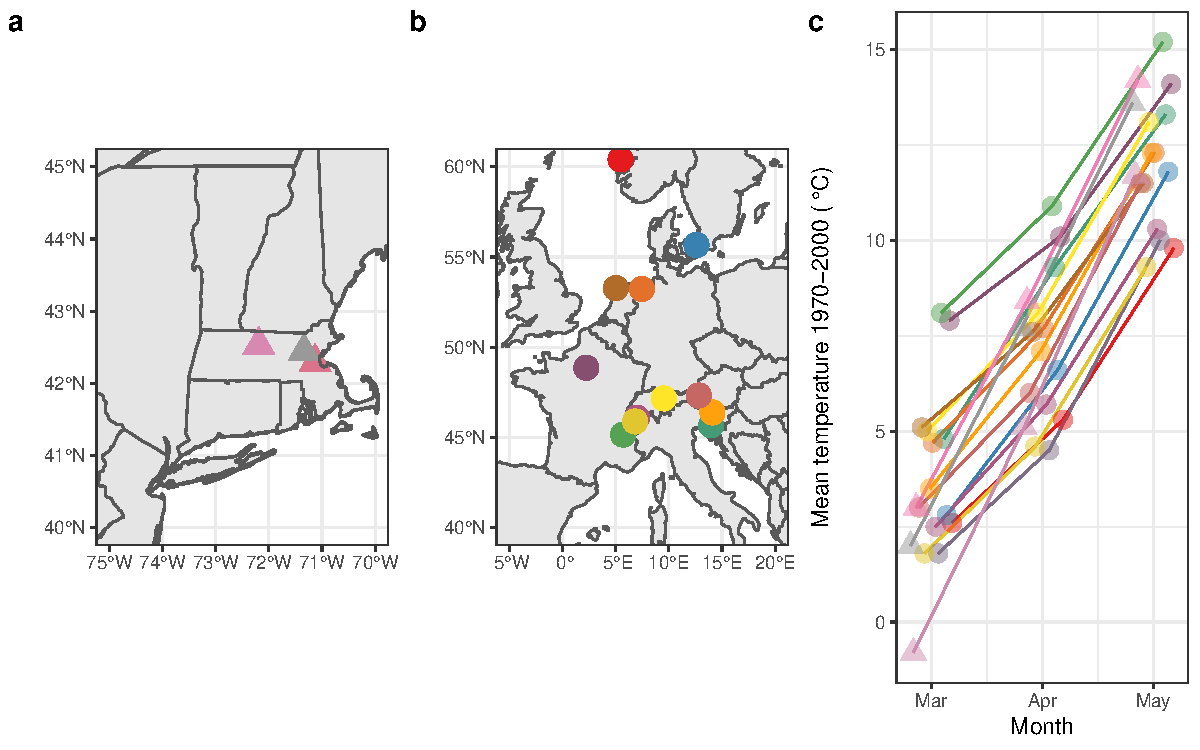
\includegraphics[width=1 \textwidth,trim=0cm 0cm 0cm 0cm, angle=0, scale=.9, origin=c,clip=false]{sampling_sites}
		\caption{Map of collection sites of (A) invasive populations in New England and (B) native populations in Europe and (C) average March, April, and May temperatures at each site. Note that spring temperature at native populations (circles) are similar to spring temperature experienced by invasive populations (triangles), but also show key differences: invasive populations are exposed to greater increases in temperature from March to May. } % This difference may be sufficient to select for later-germination. 
		\label{fig:sites}
	\end{figure}


	\subsection{Experimental Design} 
	To test phenological responses to climate, seeds were exposed to eight treatments representing varying climates. Seeds were first subjected to either a long or short stratification treatment, and then planted in one of four spring temperature treatments. All treatments were carried out in growth chambers. For each treatment, 20 representatives of each species (with seven invasive species this equals 140 seeds per treatment) and an additional five representatives of each local population of \textit{Plantago lanceolata} (the most heavily sampled species, with 13 populations) leading to a total of 205 seeds per treatment. Local population representatives were drawn from the greatest array of seed families, and seed family representation was equal across treatments. 
	
	\subsection{Stratification} 
	We stratified all seeds at 4$^\circ$C, 70\% humidity, 380 ppm of $CO_2$ \parencite[e.g.,][]{Meekins1999,Popay1970} on moistened Whatman 1 qualitative filter paper in sterile, vented, light-version Greiner bio-one 94x16 petri dishes in darkness \parencite{Baskin1998,Popay1970} in a single Biochambers TPC-19 Reach-In Growth Chamber for either 30 days (reference level) or 60 days. These two stratification treatments represent intermediate stratification lengths for our species: studies show that our species require stratification lengths between 16 days \parencite{Popay1970} and 120 days \parencite{Meekins1999}. We began the 60-day stratification treatment in late September 2015; other seeds remained in paper envelopes at room temperature until they were in turn stratified in late October 2015.  Water was added to petri dishes every 30 days.
	
	\subsection{Germination}
	On November 23, 2015, seeds from both stratification treatments were transferred into individual pots with soil (see Experimental Design, above), which were placed into four different growth chambers (three Biochambers TPC-19 and one Biochambers LTCB-19 Reach-In Growth Chamber) and subjected to four different germination treatments. Temperature varied across treatments---all other measured variables were kept constant, and treatments were rotated through growth chambers to control for unmeasured chamber effects. (Seeds that germinated during stratification were not included in the analysis, but this was a small number and unlikely to affect results.)
	
	\paragraph{Germination Temperature:} Our four treatments used temperatures between 18 and 32$^\circ$C. Optimal weed germination typically occurs at 20-30$^\circ$C \parencite{Hartmann2010,Steinbauer1957,Wulff1994,Popay1970}. We used this  sightly broader spectrum to ensure a sufficient variance in germination response.
	
	\paragraph{Thermoperiocity:} Our treatments employed daily fluctuations in temperature (thermoperiocity) of 10$^\circ$C \parencite[see e.g.,][]{Steinbauer1957, Toole1963,ISTA1954}, translating to treatment temperatures of: 18/8$^\circ$C (reference temperature), 22.67/12.67$^\circ$C (temp1), 27.33/17.33$^\circ$C (temp2), and 32/22$^\circ$C (temp3). All treatments were subjected to 8 hours at the high temperature and the remaining 16 hours at the low temperature \parencite{Baskin1998,Roberts1981,Popay1970,Probert2000}. %About 80\% of weeds studied in \textcite{Steinbauer1957} and about 75\% of cultivated seeds germinate better with thermoperiocity (i.e., daily fluctuations in temperature)\parencite{Toole1963,ISTA1954}. 

	\paragraph{Light type, period, \& luminance:} We used T5HO fluorescent lights \parencite{Toole1963}, which have a high R:FR ratio as, generally, exposure to a high R:FR ratio increases germination rates \parencite[though some studies find germination requires high R:FR ratio or is insensitive,][]{Popay1970,Pons2000,Wulff1994}. % Germination rates typically increase when seeds are exposed to light \parencite[e.g.,][]{Baskin1998,Pons2000,Popay1970}. 
We exposed all treatments to eight hours \parencite[coinciding with the higher temperature,][]{Baskin1998} of 75 micromol/m\textsuperscript{2}/second, which yielded a daily photon dosage of 2.16 mol/m\textsuperscript{2}. This amount of light should be sufficient to evoke germination response in all species \parencite{Pons1991}. Because none of our species are known to exhibit high-irradiance response and  growth chambers provide less light than normal natural conditions, we erred on the side of high light (see Supp. for additional details). 
	
	\paragraph{Planting substrate \& water:} We planted each seed in its own tray cell, on top of Fafard Growing Mix (a mixture of fine peat moss, fine perlite, and vermiculite) soil. This planting arrangement ensures light availability \parencite{Tester1987} and provides higher germination rates than filter paper \parencite{Andrews1974}. Every two days, seeds were watered until all of the soil had become wet \parencite{Steinbauer1957}; but not so much that a film of water covered the seeds \parencite{AOSA1960}.
	
	\paragraph{Germination and growth rate monitoring:}  Collection of germination and growth data was masked to population. Seeds were checked during the light period for germination every two days. Germination was defined as the growth of shoot or radical through the seed coat \parencite{Baskin1998,Popay1970}. Germination date for each seed was recorded.  Germination was monitored until 29 Jan 2016, for a total observation length of 67 days  \parencite[this is longer than the typical two-week germination trials according to][]{Baskin1998,Wulff1994}. Aboveground linear height of each seedling was measured five times: 7 Dec 2015, 15 Dec 2015, 21 Dec 2015, 4 Jan 2016, and 29 Jan 2016. On 1 Jan 2016, the plants were moved from the growth chambers to a greenhouse subject to the following conditions: natural photoperiod (approximately 10 hours of light/day), 20 to 25$^\circ$C, and 65\% humidity.
	\subsection{Statistical analysis} 
	To test for evidence of post-introduction rapid evolution across seven species, while accounting for variation due to population and seed family, we used a Bayesian multilevel modeling framework \parencite{Carpenter2017}. These multilevel models are most
robust and generally provide high power and unbiased estimates, especially for fixed effects \parencite{Paccagnella2011}. This approach yielded estimated (fixed) effects that fully incorporate these multiple levels of variance to produce overall estimates both for each species and generalized across species. 

Plant height was roughly linear with time (see Figure \ref{fig:lmgr}), so growth rate was defined as $\beta$ in the linear model: $height = \alpha + \beta*day + error $, where $error$ is normally distributed. This growth rate was calculated for each seed that germinated. For all models (growth rate, germination rate, and germination timing), stratification length, continental origin, and temperature were treated as binary fixed effects, with the full suite of 2- and 3-way interactions included. Europe, 18/8$^\circ$C, and 30 days were reference levels for origin, stratification length, and temperature, respectively; temperature was recoded as three dummy binary factors, allowing non-linear responses to temperature. Seed family was treated as a random effect, nested within sampling population, nested within species (with both random slopes and intercepts). Growth rate was modeled with a normal error distribution: 

\begin{align}
y_i  \sim &  N(\mu_i,\sigma)\\
  \mu_i =&  \alpha + \beta_1\times origin +  \beta_2 \times strat\\
          & +\beta_3\times temp1 +  \beta_4\times temp2 + \beta_5\times temp3 \notag \\
          & 
 		 + \beta_6\times origin\times strat  + \beta_7\times origin \times temp1 \notag\\ &
 		 + \beta_8\times origin \times temp2 + \beta_9\times origin \times temp3 \notag \\ &
 		 +\beta_{10}\times strat\times temp1 +\beta_{11}\times strat \times temp2 \notag \\ &
 		 + \beta_{12}\times strat \times temp3_ + \beta_{13}\times origin \times strat \times temp1 \notag\\ &
 		 +\beta_{14}\times origin \times strat \times temp2 + \beta_{15}\times origin \times strat \times temp3 )\notag
 \end{align}
 \begin{align}
 		 \intertext{Where the $\alpha$ (intercept) and $\beta$ (slope) coefficients were all specified with the same normally-distributed nested random effects ($\gamma$): seed family nested within   sampling population, nested within species---$sp[pop[sfamily[i]]]$ (not shown above). Thus, for each $\gamma$ in $[\alpha,\beta_1:\beta_{15}]$:}
 	 		\gamma_{sp[k]} \sim & N(\mu_{\gamma}, \sigma_{\gamma}) \\
 		 \gamma_{sp[pop[j]]} \sim & N(\mu_{\gamma_{sp[k]}}, \sigma_{\gamma_{sp[k]}}) \\
 		 \gamma_{sp[pop[sfamily[i]]]} \sim & N(\mu_{\gamma_{sp[pop[j]]}}, \sigma_{\gamma_{sp[pop[j]]}}) 
\end{align}


	 Where $sp = $ species, indexed with $k$, $pop =$ sampling population, indexed with $j$, $sfamily =$ seed family, indexed with $i$, and $strat$ = stratification. Germination rate was modeled similarly to growth rate, but using a binomial error distribution and logit link function, while germination timing was modeled with a Poisson error distribution and log link function. 


	All models were estimated using four chains, each with 2000 iterations (1000 devoted to warm-up), and wide priors. All models were built with Stan \parencite{Carpenter2017} using \texttt{rstanarm} version 2.17.4 \parencite{Goodrich2018} in R \parencite{Team2015}. Chain convergence was confirmed using the Gelman--Rubin statistic/$\hat{R}$ close to one \parencite{Gelman1992}. Model implementations were validated using simulated data; model fits were assessed using posterior predictive checks \parencite{Gelman2004}.  
	
	\paragraph{Average predictive comparisons:} The interactions of treatments (stratification and temperature) and random effects (species, population and seed family) make this model complex, and can make clear interpretations of parameter estimates difficult. To address this, we calculated average predictive comparisons \parencite{Gelman2007} for each stratification and  temperature level. These estimates average over interaction terms and the full mixed (fixed and random) effects, to provide a single estimate per level that includes all modeled uncertainty. Additionally, unlike model output from Poisson and Binomial models, which are given in transformed units, average predictive comparisons yield estimates that are in the units of the dependent variable (but always positive) \parencite{Gelman2007} and thus allow comparisons across effects. We note that average predictive comparisons can be complicated to implement in many unbalanced designs; because our stratification and temperature variables are balanced and independent (i.e., every combination of input values is equally likely to co-occur), we calculated average predictive comparisons without any weighting requirement, thus simplifying the computation. See Supplement for equations and details.

	\section{Results} 
	\paragraph{Germination rate:} Germination rate was high: across all species, populations, and seed families, 76\% of seeds germinated. Overall, germination rate was insensitive to stratification, temperature, or origin---95\% credible intervals (henceforth, `CrI') for all effects were clustered around zero (Figures \ref{fig:coef}, \ref{fig:rawrate}; Table \ref{tab:mod_rate}). Regardless of the climatic conditions, seeds germinated at fairly constant, high rates. Seeds from the invasive and native ranges germinated at similar rates and responded similarly to treatments (see `origin,' `strat,' `temp1,' `temp2,' `temp3,' `origin $\times$ strat,' `origin $\times$ temp1,' `origin $\times$ temp2,' `origin $\times$ temp3,' `strat $\times$ temp1,' `strat $\times$ temp2,' `strat $\times$ temp3,' `origin $\times$ strat $\times$ temp1,' `origin $\times$ strat $\times$ temp2,' `origin $\times$ strat $\times$ temp3' in Figure \ref{fig:coef} and Table \ref{tab:mod_rate}). Seeds from different local populations of \textit{Plantago lanceolata} also germinated at similar rates (see Figure \ref{fig:pops}).
 %(95\% CrI: round(invlogit(mod_rate$stan_summary[2,4]),2)--round(invlogit(mod_rate$stan_summary[2,10]),2))
	\paragraph{Germination timing:} The mean time to germination across all species, populations, and seed families was 12.33 days.   Overall, stratification and seed origin had no noticeable effect (see `origin' and `strat' in Figure \ref{fig:coef} and Table \ref{tab:mod_time}). All species germinated slower at the lowest temperature, but germinated at similar, faster speeds at the three higher temperatures, showing that temperature response is non-linear  (see `temp1,' `temp2,' and `temp3' in Figures \ref{fig:coef}, \ref{fig:rawtime}; Table \ref{tab:mod_time}). However, \textit{Plantago lanceolata} did show faster germination in response to med-low temperature $\times$ stratification interaction (see Figure \ref{fig:pops}).  Moreover, all species showed a significant positive interaction effect of origin, stratification and the higher temperature (95\% CrI: 1.05--2.9 days; see `origin $\times$ strat $\times$ temp3' in Figure \ref{fig:coef} and Table \ref{tab:mod_time}). That is, the invasive population germinated slower at the long stratification/highest temperature combination. Populations showed fairly homogeneous responses, though temperature $\times$ stratification interactions did show some inter-population variability (see Figure \ref{fig:pops}). 
	\paragraph{Growth rate:} The mean growth rate was 1.2 mm/day. Overall, growth rate was the most sensitive response variable to treatments, though it was still unaffected by population origin length or stratification \textit{per se} (see `origin' and `strat' in Figures \ref{fig:coef}, \ref{fig:rawgrowth}; Table \ref{tab:mod_gr}). Growth rate decreased at warmer temperatures for all species, but especially \textit{Dactylis glomerata} (see `temp1', `temp2', and `temp3' in Figure \ref{fig:coef}). This effect was larger for each higher temperature; this is in contrast to germination timing, where the decrease with temperature was more constant (see comparison in absolute change displayed in Figure \ref{fig:apc}). However, this decreased growth rate at high temperatures was not uniform across all treatments: for one of the higher temperatures (temp2) seeds stratified for 60 days and originating in North America (the invasive range) grew 0.74mm faster per day (95\% CrI: 0.22--1.27) than those stratified for 30 days from Europe (see `origin $\times$ strat $\times$ temp2' in Figure \ref{fig:coef} and Table \ref{tab:mod_gr}). 

\begin{figure}
	\begin{center}
	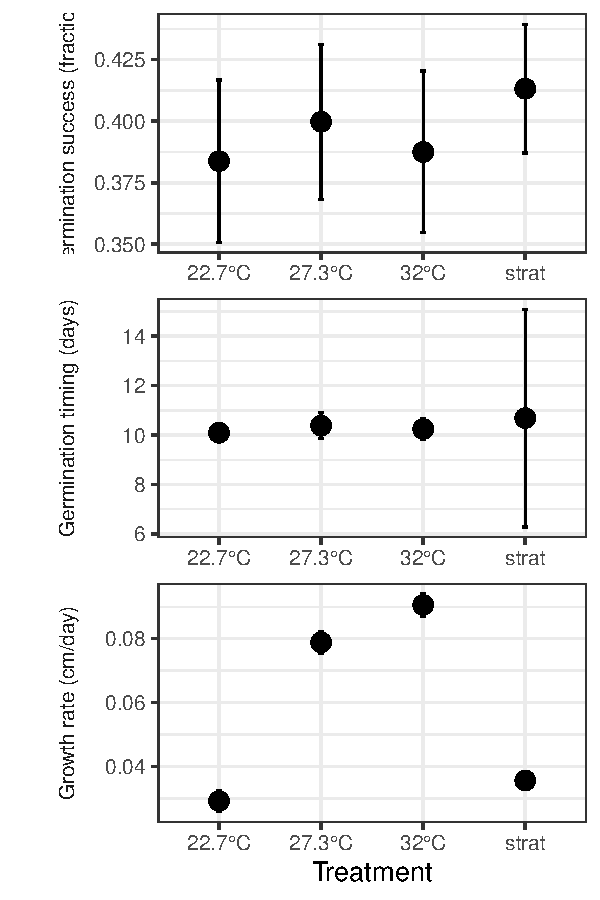
\includegraphics[width=.8\textwidth]{apc_fig.pdf}
	\caption{Average predictive comparisons ($\pm$ standard error) of germination rate (top), germination timing (middle), and growth rate (bottom) show how much change in the dependent variable results from a one unit change in the predictor variable while at once integrating over uncertainty from other effects in the model. Higher temperatures had indistinguishable effects on germination timing (middle), but sequentially bigger effects on growth rate (bottom). See Supplement for further explanation.}
\label{fig:apc}
\end{center}
\end{figure}

% latex table generated in R 3.5.1 by xtable 1.8-3 package
% Mon Jan 20 11:15:45 2020
%\begin{longtable}{rlll} 
%\label{tab:apc}\\
%	\hline
%	variable & germination rate (fraction) & germination date (days) & growth rate (mm/day) \\ 
%	\hline
%	stratification & 0.44 $\pm$ 0.02 & 9.6 $\pm$ 0.52 & 0.42 $\pm$ 0.02 \\ 
%	temperature 1 & 0.39 $\pm$ 0.03 & 10.2 $\pm$ 0.34 & 0.29 $\pm$ 0.03 \\ 
%	temperature 2 & 0.39 $\pm$ 0.03 & 10.2 $\pm$ 0.35 & 0.79 $\pm$ 0.03 \\ 
%	temperature 3 & 0.38 $\pm$ 0.03 & 10.3 $\pm$ 0.34 & 0.91 $\pm$ 0.03 \\ 
%	\hline\\
%	\hline
%\end{longtable}



\begin{figure}
	\begin{center}
		%width=1.1\textheight,
	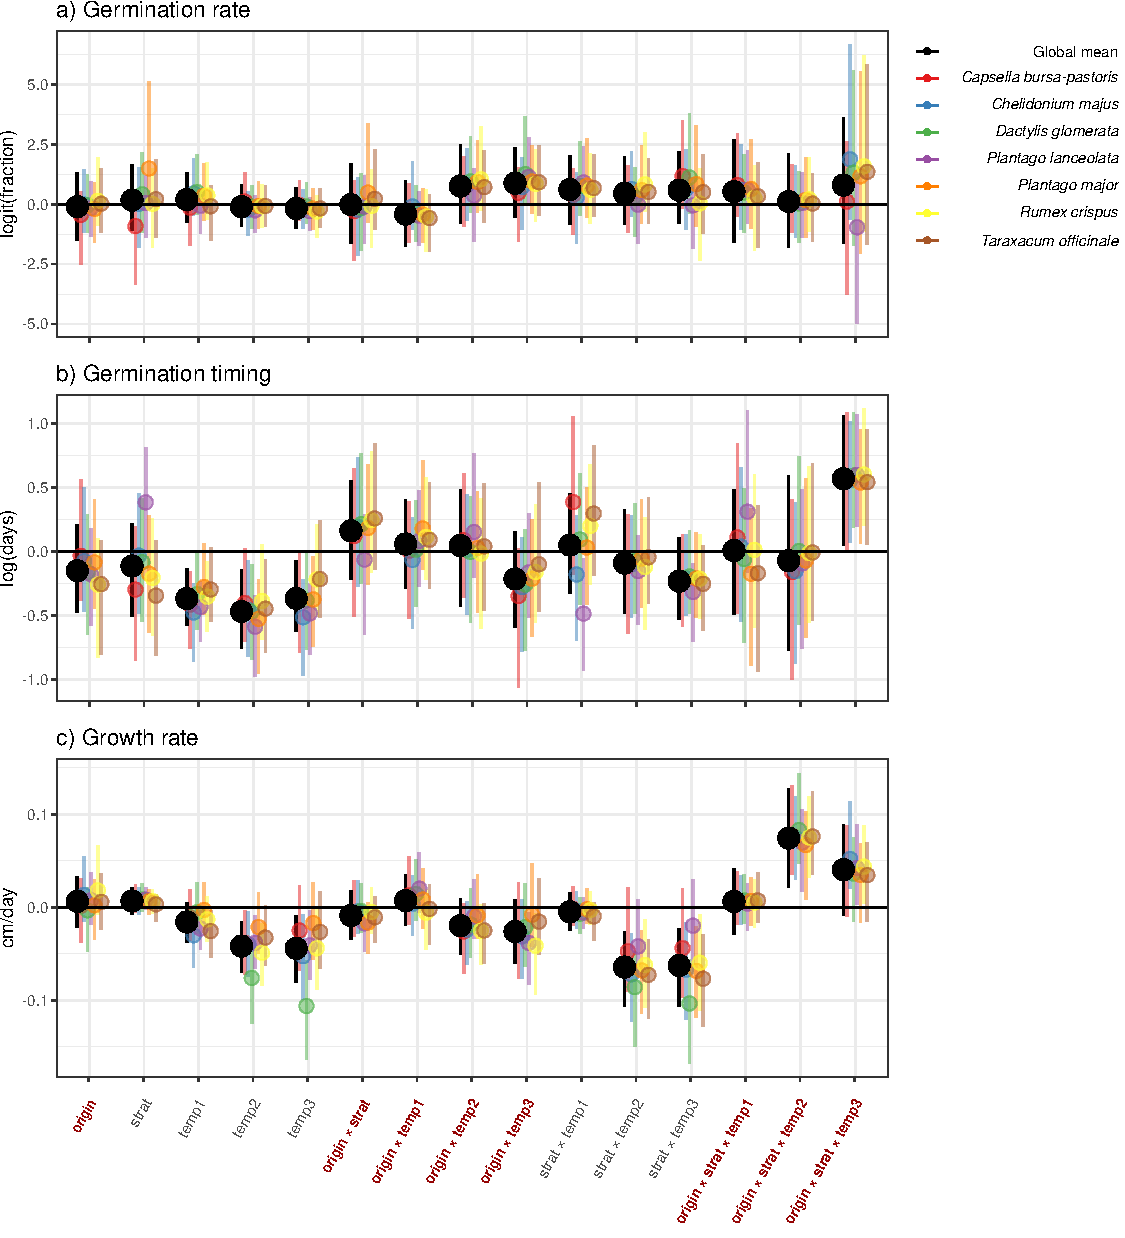
\includegraphics[ scale=1]{germ_figs_onepage.pdf}
	\caption{Multilevel model coefficients with means (circles) 95\% credible intervals (lines) for a) germination rate, b) germination timing and c) growth rate, showing overall effects across species (black circles, `global mean') and species-specific random effects (colored circles, for intercept coefficients, see Tables \ref{tab:mod_rate},\ref{tab:mod_time}, \ref{tab:mod_gr}).  The reference level for temperature is 18/8$^\circ$C, while temp1 = 22.67/12.67$^\circ$C, temp2 = 27.33/17.33$^\circ$C, and temp3 = 32/22$^\circ$C. Thirty days (30 d) is the reference level for stratification (thus, strat=60 d).}
	\label{fig:coef}

\end{center}
\end{figure}

	\section{Discussion}
	
	This study leveraged the power of a multi-species growth chamber experiment of native and introduced populations to investigate the importance of post-introduction rapid evolution for widespread plant invasions across a range of winter-to-spring climatic regimes.  All seven widespread, weedy, highly invasive plant species responded similarly to climate treatments. Across all species, we found only isolated support for the prevalence of post-introduction rapid evolution of key invasion traits---germination rate, timing, and growth rate. Instead, our results suggest that these traits do not need to evolve for these species to invade: weediness, wide environmental tolerance, plasticity, or generalist traits in the source populations may instead provide sufficient capacity to exploit novel environments \parencite{Baker1965}. Post-introduction rapid evolution may provide a helping hand, but---at least for these traits and for widespread invaders---rapid evolution does not appear generally essential for invasion success. This is an encouraging result for forecasts of invader responses to climate change as it suggest we may be able to use current estimates to extrapolate to future responses (up to a point). 
	
	The evidence for broad environmental tolerance is especially pronounced in germination rate, where all species germinated well, with little regard for climatic conditions. This result suggests that rather than evolving upon invasion, or utilizing some other mechanism, these widespread invaders drew on the broad environmental tolerance in their source populations. Given the relationship between germination success and fitness, this invariant and high germination across climates may be consistent with adaptive phenotypic plasticity \parencite{Baker1965}. Some have suggested that, while initially species may not need to evolve, they may evolve once achieving a foot-hold \parencite{Lamarque2015}. However, many of the study species (e.g., \textit{Dactylis glomerata}) have occupied their invasive range for centuries, yet still show little sign of an evolving, or evolved, germination response in our experiment. 
	
	This evidence for broad environmental tolerance suggests that these widespread invasive species may continue to perform well with continued climate change, without any evolution in these traits. This inference may hold for other widespread species, too.  Plant invasions have long been used as a natural experiment for studying plants more generally \parencite[e.g., ][]{Yoshida2007}. In that light, these results can be seen as a natural experiment of how widespread species may react to rapid climatic change, where the climate change experienced when a plant colonizes a new environment is a proxy for the anthropogenic climate change that plants are experiencing now. Thus, these results indicate that widespread plants may have the capacity to maintain their germination rates despite the changing climate. Future research should test if more localized temperate plant species share this broad environmental tolerance, or if these localized species may become inferior competitors as the climate changes. If the latter case is true, then climate change may increase the dominance of widespread species. % emw 31 Oct 2020 -- nice!

	Overall, germination timing and growth rate showed few signs of post-introduction evolution. However, there was some evidence that particular responses have evolved: North American (invasive) populations germinate later and grow faster under long stratification/high spring temperature combinations. Taking the climate of North American populations into account (Figure \ref{fig:sites}), this rapid post-introduction evolution of growth rate may be adaptive. North American populations experience climates with longer winter stratification  (lower mean March temperatures) and hotter spring temperatures (higher mean May temperature). Thus, the capacity to grow faster after being exposed to a long stratification treatment and high temperatures may provide fitness advantages. Our experimental design's inclusion of multiple seeds per seed family suggests that these results are not due to maternal effects. However, it is  possible that these differences could be due to residual founder effects \parencite{Shirk2014}, genetic drift \parencite{Eckert1996}, or between-seed family maternal effects \parencite{Galloway2005}. Nevertheless, the convergence between experienced climate and the observed change in growth rate is consistent with adaptive post-introduction rapid evolution. 
	
	These results highlight the need to condition biological invasion mechanisms on specific invasion traits \parencite{Maillet2000}. We found that post-introduction rapid evolution played no role in germination rate, but may play a role in growth rate under certain treatment conditions. This suggests that research and theory aimed at identifying which traits are likely to rapidly evolve with invasion may yield more insights than testing for an overall mechanism of invasion that is consistent across traits. We found evidence that germination timing and growth rate traits were most likely to evolve in response to specific combinations of spring temperatures and winter length. This result suggests that considering the interdependent multivariate environment in the invasive range may be critical for predicting how traits evolve post-introduction. 
%	Furthermore, the types of environmental variables in which these traits evolve in response to can also be illuminating. Our results suggest that traits are most likely to evolve in response to specific combinations of spring temperature and winter length.  Adaptation to winter length is especially under-studied, and our results suggest that examining it is most useful in concert with other climate variables.  
Not only can these trait evolution/environment relationships be useful for understanding invasions, they can also help delineate plant capacities to adapt to the multifaceted effects of anthropogenic climate change. 
	
	Our findings suggest that these invasive species may be able to adapt to changing climates by shifting germination timing or growth rate. The evidence that species can adapt their growth rate under certain conditions suggests that invasive species may have the capacity to adapt to changing winter lengths and warming spring temperatures that are expected under anthropogenic climate change \parencite{IPCC2015}. If species are adapting to specific combinations of winter $\times$ spring climatic regimes, it would make forecasting responses difficult, as forecasters would need to consider multivariate environments and include evolutionary responses. Our results also echo the importance of designing experiments that vary both winter length and spring temperature in order to observe responses to climate change \parencite[e.g.,][]{Bernareggi2016}. 

	Our results come from a limited number of individuals and populations collected from the invasive range (see Figure \ref{fig:sites}; Table \ref{tab:seeds}). The small amount of geographic variation captured in this invasive range may have introduced bias, yet our sampling sites show substantial climate variation (Figure \ref{fig:sites}), highlighting potentially important climatic differences that should provide some degree of site difference.  While additional sampling across the invasive range would have yielded greater geographical inference to our findings, it may also have made the complex stratification by temperature responses harder to detect---if such responses, and their evolution, are dependent on specific multivariate climates. Based on our findings, we suggest sampling across distinct invasive range climates could help understand which traits evolve where, post-introduction. % Such studies could leverage Bayesian modeling to include climate as a predictor, while controlling for other factors. 
	
	We harnessed the benefits of growth chambers to provide a common set of precisely controlled multivariate environments for seven species; however, the benefits of this design trade off with a lack of realism. In contrast to reciprocal field common garden experiments, which can integrate important factors \parencite{Germain2018,Blois2013}, our approach lacked most biotic interactions and natural climatic variation. Yet our approach let us tease apart the multivariate nature of climate (stratification $\times$ temperature) and examine evidence for post-introduction rapid evolution across a large range of introduced climates. We believe combining similar growth chamber designs with Bayesian modeling approaches, which integrate across multiple levels of variance (species, population, seed family), provides a tractable approach for other populations, other traits, and other combinations of climate factors (including precipitation). Such future small-scale growth chamber studies could enable robust meta-analyses capable of identifying the traits and climate responses for which post-introduction rapid evolution is, or is not, essential for invasion success, and may guide where best to invest the intensive resources required for reciprocal field common garden experiments. 
	
	Our results show that post-introduction rapid evolution of germination and growth traits is unlikely to be essential for all plant invasions and that current phenological flexibility seen in invaders was likely present in their native ranges. This suggests that broad environmental tolerance may be important for invasion success in these seven widespread invaders. Post-introduction rapid evolution may still play a role, especially in more extreme or different environments.  \textcite{Linde2001} found that \textit{Capsella bursa-pastoris} evolved to colonize high-altitude and desert environments in California. In contrast, our temperate population comparisons showed little sign of rapid evolution, suggesting the generalist traits contained in temperate source populations may be suitable as long as the introduced environment is not too different \parencite{Baker1965}. Our findings provide support for  the speculation by van Kleunen and colleagues (2010) that future invasions can be predicted by species' characteristics (such as broad environmental tolerance), but perhaps only for specific traits (such as germination rate). Consequently, managers can perhaps best guard against future invasions by targeting widespread weedy species and preventing them from dispersing beyond their native ranges. Likewise, our results suggest that current estimates of invaders' responses to diverse climates may forecast their future responses under continued climate change. 
	
\paragraph{Acknowledgments}
Thanks to E. Forrestel for mentorship to HNE. Thanks to J. Williams and H. Branch for fruitful discussions. Thanks also to D. Flynn, S. Gee, J. Samaha, and T. Savas for help transplanting, collecting, and measuring. Thanks to F. Rosin, K. Woodruff, and J. Gard for help with collection and growing logistics. Thanks to S. Fritz for help with data input. Thank you to A. Acosta, D. Buonaiuto, C. Chamberlain, A. Delgado, A. Ettinger, N. Gilbert, C. Husic, and M. Rucinski for comments on earlier drafts of this paper. Thanks to J. Eyster, S. Stalhandske, and G. Barbone for assistance with and camaraderie during field sampling. This field work was supported by the Harvard College Undergraduate Research Fund and the Harvard University Center for the Environment Undergraduate Summer Research Fund. % We also thank a number of anonymous reviewers. % emw 31 Oct 2020 -- I always add this after reviews and then delete it for submission to each new journal, may totally not be necessary though so do as you prefer!

\paragraph{Authors' contributions} HNE and EMW conceived the study and designed the methods; HNE led the data collection, analysis, and writing, with assistance from EMW. HNE and EMW contributed critically to the drafts and gave final approval for publication.

\paragraph{Data, code} 
R code, Stan code, and data will be deposited on the Knowledge Network for Biocomplexity (KNB) repository. 
\printbibliography 
\end{document}
